% Final report, HiddenStates (due 31 Oct 2026). Build:
%   pdflatex main && bibtex main && pdflatex main && pdflatex main
% Rules (course and ACL): at most 8 pages before the references; up to 2
% appendix pages after them; the limitations, challenges and future work
% section sits immediately before the references and holds no results;
% abstract at most 200 words of plain text; no em dashes; every number traces
% to a file in results/. Section owners follow docs/final-plan.md.
\documentclass[11pt]{article}
\usepackage[final]{acl}
\usepackage{times}
\usepackage{latexsym}
\usepackage[T1]{fontenc}
\usepackage[utf8]{inputenc}
\usepackage{microtype}
\usepackage{inconsolata}
\usepackage{graphicx}
\usepackage{booktabs}
\usepackage{multirow}
\usepackage{amsmath}
\usepackage{amssymb}
\usepackage{xspace}
\usepackage{xcolor}

\newcommand{\qwen}{Qwen2.5-VL-7B\xspace}
\newcommand{\llava}{LLaVA-NeXT-7B\xspace}
\newcommand{\cls}[1]{\textsc{#1}}
% Placeholder for a section not yet written; remove every use before submitting.
\newcommand{\pending}[2]{\par\noindent\fbox{\parbox{0.95\linewidth}{\small
  \textcolor{red}{\textbf{To write (#1):}} #2}}\par}

\title{Type-Aware Failure Prediction for Chart Reasoning in\\Vision-Language Models}

\author{Yash More, Naman Singhal, Shrish Kadam, Sanjith Ganapathi \\
  \texttt{\{yash.more, naman.s, shrish.kadam\}@research.iiit.ac.in}, \texttt{sanjith.ganapathi@students.iiit.ac.in} \\
  International Institute of Information Technology, Hyderabad}

\begin{document}
\maketitle

\begin{abstract}
\pending{Yash}{Abstract: at most 200 words, plain text with no LaTeX commands.}
\end{abstract}

% Introduction. Sources: results/probes/binary_*_test.md,
% results/chartqa_type_probes.md, results/labels/*.error_stats.json,
% results/synth_fabrication_pilots.md, results/pilot3_probes.md, results/e4.md,
% results/e5.md.
\section{Introduction}
\label{sec:intro}

Vision-language models (VLMs) are routinely asked to read charts, and a wrong
answer can be wrong in two different ways. The model may have \emph{misread}
the figure: taken the adjacent bar, rounded to a gridline, or misread a printed
value. The answer was in the image, and a closer look might recover it. Or it
may have \emph{fabricated}: reported a value the figure does not contain.
Looking again cannot help, and the right response is to withhold the answer.
Reliability methods usually collapse both cases into one ``do not trust''
score. We ask whether the two failure types are visible in the model's internal
state \emph{before} it answers, and whether knowing the type helps choose a
repair.

\paragraph{Problem.} Let $x=(I,q)$ be a chart image and a question, and $\hat y$
the answer a frozen VLM generates greedily. Let $h_\ell(x)\in\mathbb{R}^d$ be the
hidden state after decoder layer $\ell$ at the last prompt token, computed in the
same forward pass that produces $\hat y$. Each wrong answer has a failure type
$t$, read off $\hat y$ and the figure. We test (i) whether linear probes on
$h_\ell$ predict $\Pr(\hat y \text{ wrong})$ and $t$ better than surface features
of the input, (ii) whether a probe trained for one type also responds to the
other (cross-transfer), (iii) whether the best repair depends on $t$ (E4), and
(iv) whether a controller that uses the type beats plain selective prediction
(E5). The \textbf{Type Separability Hypothesis} states that the states before a
misread and before a fabrication are linearly distinguishable, the first being
a precision-limited perceptual failure and the second an answer ungrounded in
the image. A collapse of the two classes is a reportable outcome, not a failure
of the design.

\paragraph{Contributions.} (1) Full-depth activation caches of
\qwen and \llava on ChartQA and on three synthetic pilots, taken from the pass
that produced each answer. (2) Five-label annotations of all 1,495 ChartQA
errors of both models, with a two-person agreement check. (3) Probes that
predict wrong answers (AUROC 0.877 and 0.798) and separate misreads from
arithmetic errors on real charts (0.897 and 0.961), each against surface
baselines, residualisation, five data splits and single-question-type
controls. (4) A synthetic arm that induces fabrication: neither model refuses
questions about a missing bar, yet both encode that it is missing (AUROC 0.96 to
1.00), and the same signal fires on years outside a chart's range. (5) A
pre-registered repair experiment in which cropping rescues misreads more than
fabrications in both models, and a controller evaluated against selective
prediction.

% Owner: Yash (docs/final-plan.md, Yash task 2).
\section{Background and Related Work}
\label{sec:related}
\pending{Yash}{Start from paper/mid/main.tex Section 2 (references.bib is copied from the mid report).}

% Experimental setup. Sources: configs/inference.yaml, configs/activations.yaml,
% src/extract/{qwen,llava,cache_chartqa}.py, src/probes/*.py.
\section{Experimental Setup}
\label{sec:setup}

\paragraph{Models and inference.} We use two frozen VLMs, \qwen
\citep{bai2025qwen25vl} and LLaVA-NeXT with a Mistral-7B language model
\citep{liu2024llavanext}. Each question gets the standard ChartQA suffix
``Answer the question using a single word or phrase.'' and is decoded greedily
(at most 32 tokens) in fp16 on RTX 2080 Ti GPUs. Answers are scored by ChartQA
relaxed accuracy: numbers within 5\% of the gold, strings by exact match.

\paragraph{Activations.} Forward hooks record the residual stream after every
decoder layer during the prefill of the same \texttt{generate()} call that
produces the answer, so each vector belongs to the scored answer. We pool four
positions per layer (mean and max over image tokens, the last prompt token, and
the mean over prompt text tokens) for all 28 layers of Qwen ($d=3584$) and 32 of
LLaVA ($d=4096$). The image precedes the question and attention is causal, so
image-token states cannot depend on the question.

\paragraph{Probes.} A probe is an $L_2$-regularised logistic regression on one
pooled vector, z-scored with training-set statistics, with $\lambda$ chosen from
$\{1,10,10^2,10^3,10^4\}$. The binary probe uses a 60/20/20 split by
\emph{figure}: layer, position and $\lambda$ are chosen on validation and the test
set is scored once. Type probes, whose classes are smaller, use five folds by
figure: within each outer fold, layer and $\lambda$ are chosen by inner
cross-validation on the other folds, so every item is scored by a probe that
never saw its chart; the position is fixed to the last prompt token. We report
AUROC with 95\% intervals from a bootstrap over figures (2,000 draws), since
questions on one chart are correlated. Seed 42 throughout.

\paragraph{Baselines and controls.} Every probe is reported beside a baseline
without activations. On ChartQA this is the same probe on four surface features
(question source, question length, number of image tokens, numeric gold). We
also \emph{residualise}: regress the surface features out of the activations,
fitted on training rows only, and retrain \citep{sahoo2026linearprobes}. On
synthetic charts the baselines are a question-text classifier, the image-token
probe, and the probe on chart metadata (pilot, axis range, tick density, number
of bars, lookalike name, phrasing).

% Owner: Sanjith (docs/final-plan.md, Sanjith task 4). Sources: results/labels/,
% results/human_agreement.md.
\section{Labelling the Errors}
\label{sec:labels}
\pending{Sanjith}{Five-label taxonomy, label counts for both models, and the human agreement check (two annotators kappa 0.421; below the 0.6 gate; adjudicated human labels vs LLM kappa 0.614; results/human\_agreement.md).}

% Owner: not assigned in docs/final-plan.md (ask the team). Sources:
% results/probes/binary_*, binary_followups*, chartqa_types_*,
% results/chartqa_type_probes.md.
\section{Naturalistic Arm: ChartQA (E1 to E3)}
\label{sec:chartqa}
\pending{unassigned}{E1 binary probe with robustness checks, E2 surface and residualised baselines, E3 misread vs computation on real charts. Start from paper/mid/main.tex Section 5.}

% Synthetic arm. Sources: results/synth_fabrication_pilots.md,
% results/probes/synth_pilot2_*.json, results/probes/synth_types_*.json,
% results/synth_type_probes.md, results/probes/synth_grid_baseline_*.json,
% results/probes/transfer_chartqa_*.json, results/pilot3_probes.md,
% results/probes/pilot3_*.json. Outcome counts rescored with src/synth/items.py.
\section{Synthetic Charts: Inducing Fabrication}
\label{sec:synth}

\paragraph{Design.} We induce fabrication by asking about something the chart
does not show. Two constraints shape the design: a probe comparing ChartQA
misreads with synthetic fabrications would learn ``real vs.\ synthetic chart'',
and on synthetic data the question template alone predicts the intended failure
type perfectly. Every contrast is therefore made \emph{within one question
wording}, and every outcome is scored from the model's actual answer.
\textbf{Pilot 1} (300 bar charts, 4 to 7 bars, six themes) asks each chart the same
question twice: once about a shown bar (``What is the value of Mango?'') and once
about a plausible missing name (``\dots of Guava?''). \textbf{Pilot 2} (300
charts) adds lookalike names (asked for Dubai when Dublin is shown), values off
multiples of 5 on axes up to 200, and two more question families:
\emph{compare} (``Which is larger, Guava or Apple?'') and \emph{neighbor}
(``Which bar is right of Guava?''). \textbf{Pilot 3} (300 charts of consecutive
years) asks about a shown year and, in the same words, about a year one to three
years outside the shown range. A missing-bar answer is scored as
\emph{rejected} (``not shown''), \emph{``0''} (no bar has zero height, so we
treat it as a refusal expressed as a number, and score it wrong but not as
fabrication), \emph{fabricated} (any other number, or naming a bar), or
\emph{picked shown} (naming the shown bar in a compare question, reported
separately).

\begin{table}[t]
\centering\small\setlength{\tabcolsep}{3pt}
\begin{tabular}{llcc}
\toprule
 & & Qwen & LLaVA \\
\midrule
Shown bar, value & read right & 554/600 & 185/600 \\
\midrule
\multirow{3}{*}{Missing, value} & rejected & 15 & 0 \\
 & ``0'' & 494 & 232 \\
 & fabricated & 91 & 368 \\
\multirow{2}{*}{Missing, compare} & fabricated & 37 & 101 \\
 & picked shown & 263 & 199 \\
Missing, neighbor & fabricated & 300 & 290 \\
\midrule
\multicolumn{4}{l}{\textit{Missing-vs-shown probe, test AUROC}} \\
\multicolumn{2}{l}{\quad value} & 0.999 & 0.977 \\
\multicolumn{2}{l}{\quad compare} & 0.991 & 0.959 \\
\multicolumn{2}{l}{\quad neighbor} & 1.000 & 0.996 \\
\multicolumn{2}{l}{\quad text-only baseline} & 0.49--0.52 & 0.49--0.52 \\
\multicolumn{2}{l}{\quad image-token probe} & 0.500 & 0.500 \\
\bottomrule
\end{tabular}
\caption{Pilots 1 and 2. Top: answers (value rows pool both pilots; compare and
neighbor are pilot 2, 300 each). Bottom: probes separating a missing from a
shown name under identical wording (pilot 2, held-out charts).}
\label{tab:synth}
\end{table}

\paragraph{The models know the bar is missing, and answer anyway.}
Neither model refuses: Qwen rejects 15 of 1,200 missing-name questions and LLaVA
none (Table~\ref{tab:synth}). Qwen mostly answers ``0'', and when it invents a
number it usually copies the lookalike bar (57 of its 76 pilot-2 inventions);
LLaVA invents far more often (368 vs.\ 91). Yet probes on the last prompt token
separate missing from shown names almost perfectly, also for lookalike names
(0.98 to 1.00 Qwen, 0.92 to 0.99 LLaVA). Two controls rule out shortcuts: a
classifier on the question text is at chance, because every name is shown on
some charts and missing on others, and the image-token probe scores exactly
0.500, because image tokens precede the question and cannot see it. The signal
appears early (Qwen by layer 2, LLaVA by about layer 9).

\begin{table}[t]
\centering\small\setlength{\tabcolsep}{2.5pt}
\begin{tabular}{lcccccc}
\toprule
 & \multicolumn{3}{c}{Qwen} & \multicolumn{3}{c}{LLaVA} \\
Probe & S/C & F/C & F/Z & S/C & F/C & F/Z \\
\midrule
Misread (S/C) & \textbf{.887} & .594 & .400 & \textbf{.776} & .879 & .215 \\
\quad metadata & .814 & .557 & .543 & .512 & .522 & .537 \\
\quad + gridline$^\dagger$ & .920 & & & .860 & & \\
Fabricated (F/C) & .576 & \textbf{1.00} & .286 & .680 & \textbf{.988} & .243 \\
Invented vs.\ ``0'' & .336 & .138 & \textbf{.984} & .520 & .226 & \textbf{.986} \\
\bottomrule
\end{tabular}
\caption{E3 cross-transfer on synthetic value questions (pilots 1 and 2, 5-fold
CV by chart). Rows: the probe; columns: the contrast it is scored on (C correct
read, S misread, F invented number, Z ``0''). Bold: own task. Metadata: the
same probe on chart settings. $^\dagger$Gridline features chosen after seeing
the data.}
\label{tab:matrix}
\end{table}

\paragraph{Misreads vs.\ fabrications (E3).} On the value template the four
classes are correct read, misread, invented number and ``0'' (Qwen 554, 46, 91,
494; LLaVA 185, 415, 368, 232). In Qwen the two type probes are largely specific
(Table~\ref{tab:matrix}): the misread probe barely responds to fabrications
(0.594), and the fabrication probe barely to misreads (0.576). In LLaVA the
misread probe fires \emph{more} on fabrications (0.879) than on its own task
(0.776), the pattern our proposal called one signal wearing two labels. In both
models the ``fabrication'' probe is a missing-bar detector: it ranks ``0'' answers
as high as invented numbers. What separates an invented number from ``0'' is
decodable (0.984 and 0.986), but only in the last layers, where it reads out the
answer about to be produced (Appendix~\ref{app:layers}).

\paragraph{A chart property explains synthetic misreads.} Relaxed accuracy
tolerates a 5\% \emph{relative} error, so whether a coarse reading is a misread
depends on how far the true value lies from a gridline relative to its size. Two
features declared in advance (distance to the nearest gridline, and to the
nearest multiple of 10) added to the metadata reach 0.853 (Qwen) and 0.642
(LLaVA), below both probes; the same distances divided by the value, added after
seeing that result, reach 0.920 and 0.860, above both. Synthetic misread probes
also transfer poorly to real charts: trained on synthetic charts and applied
unchanged to ChartQA, they separate real misreads from correct answers at only
0.597 (Qwen) and 0.557 (LLaVA). The synthetic misread signal may describe the
chart more than the model.

% Generated by scripts/final_assets.py from results/probes/pilot3_*.json
% See results/pilot3_probes.md. Caption: PILOT3_CAPTION in the script.
\begin{table}[t]
\centering\small
\setlength{\tabcolsep}{2pt}
\begin{tabular}{lcc}
\toprule
 & Qwen & LLaVA \\
\midrule
\multicolumn{3}{l}{\textit{Answer to the out-of-range year}} \\
Refused & 102 & 0 \\
``0'' & 76 & 19 \\
Made-up number & 105 & 281 \\
Unclear & 17 & 0 \\
\textit{Shown year read correctly} & 273 & 74 \\
\midrule
\multicolumn{3}{l}{\textit{Missing-vs-shown probe}} \\
\quad layer & L10 & L18 \\
\quad out-of-range vs.\ shown & 1.000 {\scriptsize[1.00, 1.00]} & 0.911 {\scriptsize[0.89, 0.93]} \\
\quad made-up vs.\ correct & 1.000 & 0.922 \\
\quad made-up vs.\ refused & 0.521 & -- \\
\quad misread vs.\ correct & 0.494 & 0.568 \\
\multicolumn{3}{l}{\textit{Fabrication probe (E3)}} \\
\quad layer & L10 & L19 \\
\quad out-of-range vs.\ shown & 1.000 {\scriptsize[1.00, 1.00]} & 0.880 {\scriptsize[0.85, 0.90]} \\
\bottomrule
\end{tabular}
\caption{Pilot 3: each chart is asked about a shown year and, in the same
words, about a year outside the shown range. Top: what the models answered to the
out-of-range year (300 per model). Bottom: AUROC of the two missing-bar probes,
trained on pilots 1 and 2 only and applied unchanged, with 95\% figure-bootstrap
CIs; layer chosen on pilots 1 and 2.}
\label{tab:pilot3}
\end{table}


\paragraph{The missing-bar signal is about answerability (pilot 3).} In pilots 1
and 2 a fabrication always concerns a missing category. Pilot 3 separates the two
(Table~\ref{tab:pilot3}). Here Qwen refuses 102 of 300 out-of-range years, against
15 of 1,200 missing names, while LLaVA still invents a number for 281. Most
invented numbers copy a shown bar's value (92 of 105 for Qwen, 135 of 281 for
LLaVA) rather than extend the trend (5 and 9). Both missing-bar probes, trained
only on missing \emph{names} in pilots 1 and 2, flag out-of-range \emph{years}
perfectly in Qwen and at 0.911 and 0.880 in LLaVA, are at chance in the first
layers, and ignore misreads of shown years. In Qwen the probe fires equally
whether the model then refuses, says ``0'' or invents a number (invented vs.\
refused 0.521): it encodes that the chart cannot answer the question, not what
the model will do about it.

% Naman's sections of the final report: E4, E5 and the discussion.
% Structure only. Every paragraph below is for Naman to write (the course
% requires the report text to be written by the team). Each TODO names the
% result file holding its facts; every number must match that file.
% Tables and figure: regenerate with `python scripts/final_assets.py`.

\section{Does the failure type decide the repair? (E4)}
\label{sec:e4}

% TODO (Naman): setup. What was re-asked (every value-question error of
% synthetic pilots 1 and 2: Qwen 631, LLaVA 1,015), the four repairs, how a
% repair counts as a recovery, and the pre-registered test.
% Facts: results/e4.md (Provenance), results/e4-preregistration.md.

% Generated by scripts/final_assets.py from results/e4/*.outcomes.jsonl
% Pilots 1 and 2 pooled; see results/e4.md. Caption: E4_CAPTION in the script.
\begin{table}[t]
\centering\small
\setlength{\tabcolsep}{3pt}
\begin{tabular}{lrcccc}
\toprule
Original answer & $n$ & Re-ask & Upsample & Crop & Verify \\
\midrule
\multicolumn{6}{l}{\textit{Qwen2.5-VL-7B}} \\
Misread & 46 & 0.11 & 0.13 & \textbf{0.26} & 0.09 \\
Made-up number & 91 & 0.00 & 0.00 & 0.00 & \textbf{0.14} \\
``0'' & 494 & 0.02 & 0.02 & 0.02 & \textbf{0.69} \\
\quad crop DiD & & \multicolumn{4}{c}{+0.261 [+0.140, +0.389]} \\
\midrule
\multicolumn{6}{l}{\textit{LLaVA-NeXT-7B}} \\
Misread & 415 & 0.03 & 0.01 & \textbf{0.15} & 0.03 \\
Made-up number & 368 & 0.00 & 0.00 & 0.00 & 0.00 \\
``0'' & 232 & 0.00 & 0.00 & 0.00 & 0.00 \\
\quad crop DiD & & \multicolumn{4}{c}{+0.152 [+0.119, +0.189]} \\
\bottomrule
\end{tabular}
\caption{E4 recovery rates on initially wrong value answers. Bold marks each
row's best repair, excluding zero ties. DiD compares crop's recovery gain on
misreads with its gain on made-up numbers. Brackets give 95\% CIs from figure
bootstraps; missing-bar ``0'' answers form a separate row.}
\label{tab:e4}
\end{table}


% TODO (Naman): result of the pre-registered test, both models (Table~\ref{tab:e4}).
% Facts: results/e4.md, Qwen and LLaVA sections.

% TODO (Naman): what limits the reading. Facts: results/e4.md,
% "Read these before writing them up", points 1 to 5.

\section{A type-aware controller (E5)}
\label{sec:e5}

% TODO (Naman): setup. The policies compared, how a re-look is priced on right
% answers (the re-ask of correct answers), cross-fitting by figure fold, AURC.
% Facts: results/e5.md, and src/controller/e5.py docstring for the method.

% Generated by scripts/final_assets.py from results/e5/*_e5.json
% (see results/e5.md). AURC: mean risk over the risk-coverage curve, lower
% is better; brackets are 95% cluster-bootstrap intervals.
% Caption: E5_CAPTION in the script.
\begin{table}[t]
\centering\small
\setlength{\tabcolsep}{3pt}
\begin{tabular}{lcc}
\toprule
Policy & AURC & 95\% CI \\
\midrule
\multicolumn{3}{l}{\textit{Qwen2.5-VL-7B}} \\
Plain model & 0.526 & [0.513, 0.538] \\
Binary abstention & 0.179 & [0.169, 0.190] \\
Missing-bar abstention & 0.208 & [0.191, 0.226] \\
Controller & 0.162 & [0.145, 0.180] \\
Re-look + binary & 0.114 & [0.103, 0.126] \\
Oracle & 0.056 & [0.049, 0.064] \\
\quad re-look gain (binary) & $-$0.065 & [$-$0.073, $-$0.056] \\
\quad re-look gain (missing-bar) & $-$0.045 & [$-$0.054, $-$0.037] \\
\midrule
\multicolumn{3}{l}{\textit{LLaVA-NeXT-7B}} \\
Plain model & 0.846 & [0.827, 0.864] \\
Binary abstention & 0.645 & [0.608, 0.681] \\
Missing-bar abstention & 0.725 & [0.686, 0.759] \\
Controller & 0.715 & [0.674, 0.750] \\
Re-look + binary & 0.638 & [0.600, 0.674] \\
Oracle & 0.497 & [0.464, 0.528] \\
\quad re-look gain (binary) & $-$0.007 & [$-$0.012, $-$0.003] \\
\quad re-look gain (missing-bar) & $-$0.010 & [$-$0.017, $-$0.005] \\
\bottomrule
\end{tabular}
\caption{E5 AURC on 1,200 value questions per model, with 95\% figure-bootstrap
CIs. Each re-look gain compares policies with the same abstention ranking:
re-look plus binary minus binary, or controller minus missing-bar abstention.
A negative difference means re-looking helps. The oracle uses true classes.}
\label{tab:e5}
\end{table}


\begin{figure}[t]
\centering
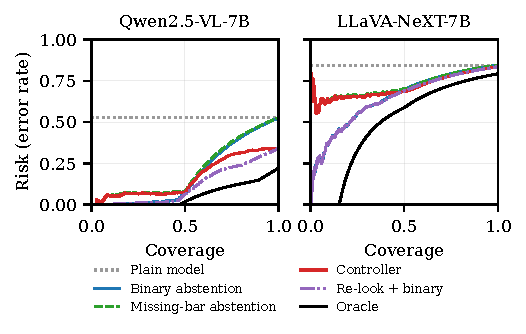
\includegraphics[width=\columnwidth]{figures/e5_risk_coverage.pdf}
\caption{TODO}
\label{fig:e5}
\end{figure}

% TODO (Naman): results (Table~\ref{tab:e5}, Figure~\ref{fig:e5}).
% Facts: results/e5.md tables and the per-class re-look breakdown.

% TODO (Naman): what the re-look actually fixes, and the oracle gap.
% Facts: results/e5.md, "Read these before writing them up", points 1 to 5.

\section{Discussion}
\label{sec:discussion}

% TODO (Naman): is the type separability hypothesis supported, now that E4 and
% E5 are in. Inputs: E3 (results/synth_type_probes.md,
% results/chartqa_type_probes.md), E4 and E5 above, and pilot 3 once Yash's
% probe results are in.

% Conclusion. Sources as in the sections above.
\section{Conclusion}
\label{sec:conclusion}

Before a VLM answers a chart question, a linear probe on its last prompt token
predicts whether the answer will be wrong, beyond what the question's surface
reveals. On real charts the errors are misreads and arithmetic slips, and the two
leave different internal signatures in both models. Fabrication is rare on real
charts but easy to induce: both models encode that a question asks for something
the chart does not show, and answer anyway. That answerability signal, together
with a general error score, is the most useful input for deciding when to
abstain; whether to re-look depends on the failure type, as the pre-registered
crop test shows, but in our controller re-looking helped mainly by turning
missing-bar answers into refusals.

% Owner: Sanjith (docs/final-plan.md, Sanjith task 4). Course rule: challenges,
% limitations and future work only, immediately before the references, with no
% results. Naman's E4/E5 fragment is included below.
\section*{Limitations, Challenges and Future Work}
\label{sec:limits}
\pending{Sanjith}{Merge the labelling and synthetic-arm limitations with the E4/E5 text below.}

% Handoff text for the team's single limitations section, owned by Sanjith.
% Include or merge this prose immediately before references, outside the
% eight-page main-text budget. This fragment contains no empirical results.
E4 and E5 use synthetic bar charts and a single value-question template.
Our crop requires bar geometry that the ChartQA setup does not provide. The
balanced shown-bar and missing-bar design differs from the frequency of
unsupported questions in natural chart use, so the controller AURCs should
not be extrapolated to ChartQA. Rare failure classes need larger evaluation
sets. Cross-fitting by figure still reuses the same synthetic pilots; we need
an independent domain to test generalisation. We compare answer quality and
coverage without optimising latency or inference cost. Future work should
test repair selection on naturalistic unsupported questions and extend the
analysis to node-link diagrams.



% Temporary: lists every reference until the sections cite them. Remove once
% the related work section is in, so only cited works appear.
\nocite{*}
\bibliography{references}

\clearpage
\appendix
% Appendix: at most 2 pages after the references. Sources: results/labels/,
% results/probes/binary_*_test.json, results/probes/synth_types_*.json,
% requirements.txt, configs/inference_synth_pilot*.yaml, README.md.
\section{Examples of the error labels}
\label{app:examples}

Examples from Qwen's labels, with the annotator's rationale paraphrased.
\cls{structural}: a pie chart with seven labelled sectors counted as six; the
adjacent 2017 bar reported for the asked 2018 bar. \cls{computation}: every input
printed and readable but the operation wrong, e.g.\ a ratio of levels (83/11)
where the question asks for a ratio of changes. \cls{not\_an\_error}: 0.95 for a
gold of 95\%, or a correct ratio 28/19 = 1.474 where the gold 1.18 matches no ratio
on the chart. \cls{ambiguous}: both gold and model wrong, or a question with
several readings that the model fits none of. \cls{fabrication} (Qwen's only
case): pie slices of 35, 40, 13 and 11, gold 75, model 55, which matches no slice
and no sum.

\section{Layer profiles}
\label{app:layers}

Figure~\ref{fig:binary} shows the binary probe by relative depth: the last
prompt token rises from about 0.70 at the first layer to a plateau over the last
third of each network (best at layer 21 of 28 for Qwen, 24 of 32 for LLaVA), while
image-token positions stay at 0.62 to 0.68, near the surface baseline. For chart
errors the informative state is the one that has read the question, unlike HALP's
finding for object hallucination \citep{kogilathota2026halp}.
Figure~\ref{fig:types} shows the synthetic type probes: the missing-bar signal
saturates early (Qwen by layer 3, LLaVA by about layer 8), the misread signal
builds gradually and peaks in the last third.

\begin{figure}[h]
\centering
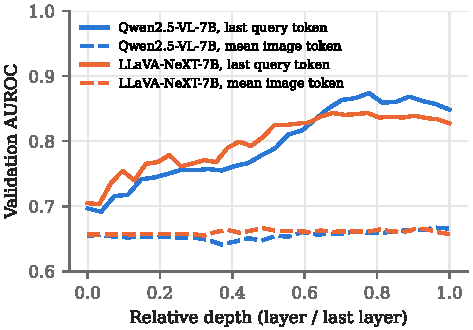
\includegraphics[width=\columnwidth]{figures/binary_by_layer.pdf}
\caption{E1 binary probe, validation AUROC by relative depth. Solid: last prompt
token; dashed: mean over image tokens.}
\label{fig:binary}
\end{figure}

\begin{figure}[h]
\centering
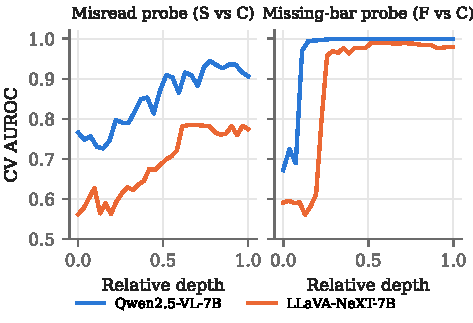
\includegraphics[width=\columnwidth]{figures/type_probes_by_layer.pdf}
\caption{Synthetic type probes, out-of-fold AUROC on their own task by relative
depth.}
\label{fig:types}
\end{figure}

\section{Reproducibility}
\label{app:repro}

All runs used RTX 2080 Ti GPUs in fp16 with SDPA attention, PyTorch 2.8.0,
Transformers 4.57.6 and seed 42, with greedy decoding of at most 32 new tokens;
the full environment is pinned in \texttt{requirements.txt}. Synthetic charts
are rendered with Matplotlib 3.10.0 and are deterministic given the seed; the
SHA-256 hashes of the three manifests (pilots 1 to 3) begin \texttt{20e80119},
\texttt{41fc27e5} and \texttt{ed311841}. Activations are pooled in fp16 and kept
off the repository. Every number in this report is read from a file in
\texttt{results/}, and the repository README lists the command that produces
each file.


\end{document}
